\documentclass[border=1pt]{standalone}
\usepackage{tikz}
\usetikzlibrary{intersections, decorations.pathreplacing, calc}


\begin{document}
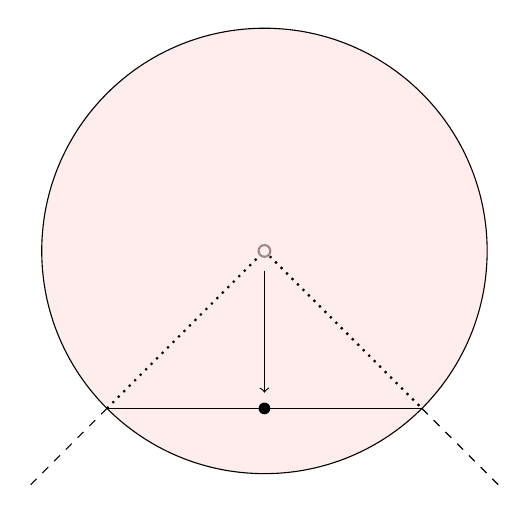
\begin{tikzpicture}[every node/.style={scale=1.5}]
  \node[opacity=.2, draw=black, densely dotted, fill=white, circle, inner sep=1pt] (x) at (0,0) {};
  \node[draw=black, thick, opacity=.4, fill=white, circle, inner sep=1pt] (x) at (0,0) {};

  % Radius of the ball
  \pgfmathsetmacro{\r}{2*sqrt(2)}

  % Draw the circle
  \filldraw[fill=red!70!white, fill opacity=.1, draw=black] (x) circle (\r);

  % Use a 45-45-90 triangle for the edges
  \coordinate (side1end) at (-2, -2);
  \coordinate (side2end) at (2, -2);

  \draw[thick, dotted] (side1end) -- (x) -- (side2end);


  % Extend them past our epsilon ball with dotted segments
  \coordinate (side1ext) at (-3, -3);
  \coordinate (side2ext) at (3, -3);

  \draw[dashed] (side1end) -- (side1ext);
  \draw[dashed] (side2end) -- (side2ext);


  \draw (side1end) -- (side2end);


  \node[fill=black, circle, inner sep=1pt] (xnew) at (0,-2) {};

  \draw[->] ($(x) + (0,-.25)$) -- ($(xnew) + (0,.2)$);



\end{tikzpicture}
\end{document}
